\documentclass[10pt,a4paper]{article}
%% Language and font encodings
\usepackage[british]{babel}
\usepackage[utf8]{inputenc}
\usepackage[T1]{fontenc}
%% Sets page size and margins
\usepackage[a4paper,top=2cm,bottom=2cm,left=2.5cm,right=2.5cm,marginparwidth=1.5cm]{geometry}
%% Useful packages
\usepackage{amsmath}
\usepackage{graphicx}
\usepackage[colorinlistoftodos]{todonotes}
\usepackage[colorlinks=true, allcolors=blue,]{hyperref}
\usepackage{authblk}
\usepackage[backend=biber,style=numeric-comp]{biblatex}
\usepackage{listings}
\usepackage{xcolor}
\usepackage{amsmath} \allowdisplaybreaks% lets align equations break over pages.
\usepackage{amssymb}

\definecolor{codegreen}{rgb}{0,0.6,0}
\definecolor{codegray}{rgb}{0.5,0.5,0.5}
\definecolor{codepurple}{rgb}{0.58,0,0.82}
\definecolor{backcolour}{rgb}{0.95,0.95,0.92}


% \addbibresource{references.bib}

\lstdefinestyle{mystyle}{
  backgroundcolor=\color{backcolour}, 
    commentstyle=\color{codegreen},
    keywordstyle=\color{magenta},
    numberstyle=\tiny\color{codegray},
    stringstyle=\color{codepurple},
    basicstyle=\ttfamily\footnotesize,
    breakatwhitespace=false,         
    breaklines=true,                 
    captionpos=b,                    
    keepspaces=true,                 
    numbers=left,                    
    numbersep=5pt,                  
    showspaces=false,                
    showstringspaces=false,
    showtabs=false,                  
    tabsize=2
}
\lstset{style=mystyle}

\graphicspath{{./img/}}

%% Title
\title{
  {\Huge Simulation and Performance Evaluation}\\
  \huge Homework 2 \\
}

\author{Blascovich Alessio and Di Noia Matteo}

\begin{document}

\maketitle

\section*{Exercise 1}

As suggested we started by setting as parameter \(N=T\lambda\) with \(\lambda = 200\) and \(T = 1000\). Then we sampled \(N\) variates from a uniform distribution in the interval \([0,T]\), that gave us the arrival times. We also sampled \(N\) variates from an exponential distribution with parameter \(\lambda\), that gave us the inter-arrival times.
\subsubsection*{From Uniform to Exponential}
Starting from the uniform \(U\sim\text{Uni}(0, T)\). We derived the distribution of inter-arrival times by sorting the extracted values and then, by computing:
\begin{equation*}
  \forall i\in[0,N]\quad from\_uni_{i} =
  \begin{cases}
    u_{i} & \text{if}\ i = 0\\
    u_{i} - u_{i-1} & \text{if}\ i\geq 1
  \end{cases}
\end{equation*}
We had to sort the extracted values because, we wanted to calculate the inter-arrival times between two adjacent events.

By plotting~\ref{fig:1}, we compared the obtain distribution against the original inter-arrival exponential distribution, and concluded that the two distributions were empirically congruent except from a small margin of error.

\begin{figure}[h]
  \centering
  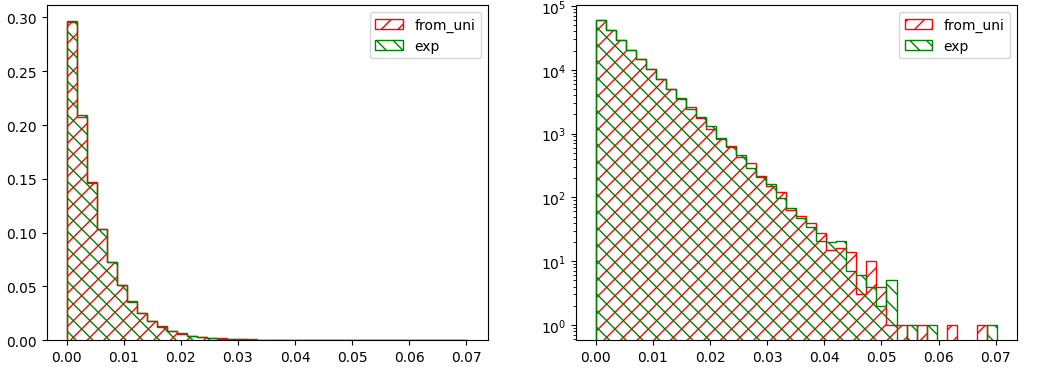
\includegraphics[scale=0.5]{es1-1.png}
  \caption{Exponential distributions}
  \label{fig:1}
\end{figure}

On the left there is the unscaled graph of the two distributions overlapping perfectly for small \emph{u}'s. To emphasise the small errors we used, on the right graph, a logarithmic scale to represent the two exponential distributions. With this representation we saw that the errors were clustered, mostly, on larger values of \emph{u}. This result was expected since, higher values of \emph{u} had a lower sample rate.

\subsubsection*{From Exponential to Uniform}

Starting from the exponential \(E\sim\text{Exp}(\lambda)\). We derived the distribution of arrival times by, for each sample compute the cumulative sum; up to that point.

\begin{equation*}
  \forall i\in[0,N]\quad from\_exp_{i} =\sum_{j=0}^{i}{e_{j}}
\end{equation*}
Note that, we had to filter out all values greater than \emph{T}, this reduced the data usable for the new exponential distribution by a \(0\%-0.2\%\). %Following the domain of the exponential distribution could be the case that, every value is bigger than \emph{T}, this is an extremely unlucky but nevertheless still possible.

\begin{figure}[h]
  \centering
  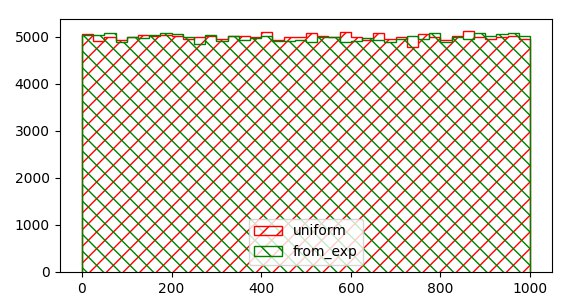
\includegraphics[scale=0.5]{es1-2.png}
  \caption{Uniform distributions}
  \label{fig:2}
\end{figure}

By plotting~\ref{fig:2}, we compared the obtain distribution against the original arrivals uniform distribution, and concluded that the two distributions are empirically congruent except from a small margin of error. In this case the error seems to be slightly bigger w.r.t.\ the previous plot.

\subsubsection*{Conclusions}

%With these two simulations we concluded that, the two methods are equivalent ways to extract a Poisson process, fixed the number of arrivals. However, the original uniform will always give exactly \emph{T} values, while the extracted exponential could be smaller. 

Variating the value \(N\) as \(N=2T\lambda\). We noticed a few changes in the simulations:
\begin{itemize}
\item The uniform distribution has twice many valid samples as the uniform generated from the exponential, this phenomenon is visible on the leftmost graph in~\ref{fig:3};
\item The exponential distribution extracted from the uniform plunges twice as fast as the original exponential, as visible in the last two graphs in~\ref{fig:3}.
\end{itemize}

\begin{figure}[h]
  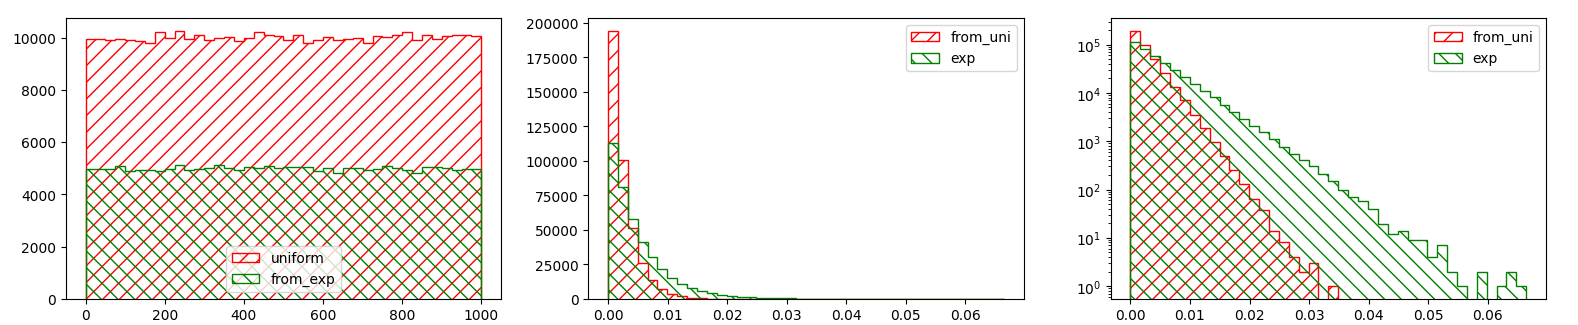
\includegraphics[scale=0.4]{es1-3.png}
  \caption{Distributions with \(N=2T\lambda\)}
  \label{fig:3}
\end{figure}

In general this can be generalised to any factor \(k\in\mathbb{N}^{+}\)

\section*{Exercise 2}

\subsubsection*{Sub-point 1}

Because for the ``rejection sample'' method any scale factor is superfluous since it only cares that the given function is bounded in its domain, we ignored the parameter \emph{A}. For the rest of the ``rejection sampling'' we used \(f^{n}(x)\) defined as \(f(x) = \frac{1}{A}f^{n}(x)\).

As bounding function we used \(g(x) = 6.36\); this function represent the maximum of the \(f^{n}(x)\) in its domain. Using this bounding function the average number of attempts to get a valid sample is:
\begin{equation*}
  \frac{\int^{3}_{-3}{g(x)}}{\int^{3}_{-3}{f^{n}(x)}}\approx4.31283
\end{equation*}

\begin{lstlisting}[language=python]
while True:
    x = float(np.random.uniform(-3, 3, 1)[0])
    u = float(np.random.uniform(0, 6.36, 1)[0])
    if u <= weird_function(x):
        return x
\end{lstlisting}
In this snippet of code \texttt{weird\_function} represents \(f^{n}(x)\).%

\subsubsection*{Sub-point 2}

\begin{figure}[h]
  \centering
  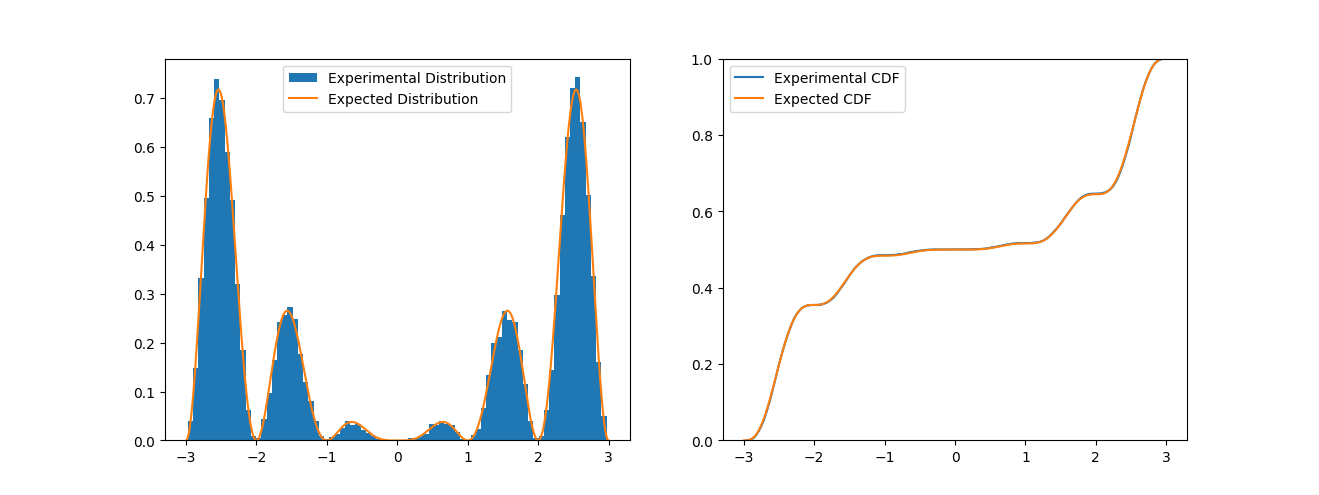
\includegraphics[scale=0.5]{es2.png}
  \caption{``Weird'' PDF and CDF}
  \label{fig:4}
\end{figure}
To have a sample for the following sub point we drawn \(20000\) variates already in this stage of the simulation.

Observing~\ref{fig:4}, on the left there are the \textbf{normalised} draws obtained by the ``rejection sampling'' compared against the real shape of \(f(x)\). With more draws the result could have been better fitting the real curve, but with this batch the fitting was already evident.

For the CDFs the non-overlapping parts are so small that they are barely visible without zooming on a particular area of the graph.

\subsubsection*{Sub-point 3}

For the median and the 0.9-quantile we used the method explained in class since we had a large \emph{n} and all the variables were IID. So we sorted the sub-sample and we used the standard value \(\eta = 1.96\), give the fact that the we were asked for \(95\%\) confidence intervals, i.e., \(\gamma = 0.95\).

\begin{lstlisting}[language=python]
def es3quantile(arr_sorted: list, q: float): # for the median q = 0.5
    n = len(arr_sorted)
    quant = np.quantile(arr_sorted, q)
    low = math.floor(n * q - ETA95 * math.sqrt(n * q * (1 - q)))
    up = math.ceil(n * q + ETA95 * math.sqrt(n * q * (1 - q)) + 1)
    ci_boot = bootstrap_procedure(arr_sorted, 25, 0.95, lambda arr: np.quantile(arr, q))
    print(...)
\end{lstlisting}

For the mean we used the asymptotic method because we had a large \emph{n} and non-wild distribution. So we computed arithmetic mean \(\mu_{n}\) and standard deviation \(s_{n}\) then we obtained the interval \(\mu_{n}\pm \eta\frac{s_{n}}{\sqrt{n}}\), with \emph{n} the size of the sample.

For the ``boostrap'' method we used an higher-order function and the standard value \(r_{0} = 25\).
\begin{lstlisting}[language=python]
def bootstrap_procedure(array: list, r0: int, gamma: float, st_func):
    r = math.ceil(2*r0/(1-gamma))-1
    stat_calculated = []
    for _ in range(r):
        draws = np.random.choice(array, len(array))
        stat_calculated.append(st_func(draws))
    stat_calculated.sort()
    return stat_calculated[r0], stat_calculated[r + 1 - r0]
\end{lstlisting}
The function takes in input the sample \texttt{array}, the value \texttt{r0}, the probability \texttt{gamma} and the function \texttt{st\_func} describing the parameter the parameter to estimate.

\subsubsection*{Sub-point 4}

Since every disjointed set is formed by \(200\) values we decided to use the asymptotic estimation as done before for the mean. Depending on the run, the percentage of sets with an arithmetic mean within the confidentiality interval was \(95\%\pm5\%\) (most of the cases). Which is expected as it is around the confidence level of the confidence interval.
\end{document}
